
%(BEGIN_QUESTION)
% Copyright 2009, Tony R. Kuphaldt, released under the Creative Commons Attribution License (v 1.0)
% This means you may do almost anything with this work of mine, so long as you give me proper credit

The Allen-Bradley model 1746-IB8 is an eight-channel discrete (on/off) input module designed for their ``SLC'' line of programmable logic controllers (PLCs).  This particular input module is designed to {\it sink} DC current originating from a 24 volt power supply (through discrete sensing devices such as pushbutton switches, toggle switches, proximity switches, and process switches).  This means the current, traced using conventional flow notation, will be seen to {\it enter} each respective channel terminal on the input module.

$$\includegraphics[width=15.5cm]{i03828x01.eps}$$

Sketch connecting wires such that the three toggle switches (A, B, and C) connect to input channels IN2, IN5, and IN7, respectively:

\underbar{file i03828}
%(END_QUESTION)





%(BEGIN_ANSWER)


%(END_ANSWER)





%(BEGIN_NOTES)

Bear in mind that this is not the {\it only} possible circuit solution:

$$\includegraphics[width=15.5cm]{i03828x02.eps}$$

%INDEX% Pictorial circuit review (PLC discrete DC input wiring)

%(END_NOTES)


